
% Hemera's Dawn chapter -----------------------------------------------
\chapter*{Hemera's Dawn}
\addcontentsline{toc}{chapter}{Hemera's Dawn}

\begin{flushright}
\parbox{0.8\textwidth}{
\emph{Then assuredly the world was made, not in time, but simultaneously with time. \\
\hspace*{\fill}{\textperiodcentered \textperiodcentered \textperiodcentered \hspace*{0.2em} St. Augustine} } }
\end{flushright}

\noindent
Hemera's Dawn is chess variant which is played on 20 x 20 board, with
darkish red-brown and gray fields and bright red and dark gray pieces.
Star colors are white and bright blue. In algebraic notation, columns
are enumerated from 'a' to 't', and rows are enumerated from '1' to '20'.
A new piece is introduced, Centaur.

\textbf{\huge{TODO :: Star colors !!!}} % TODO :: FIX ME !!!

\clearpage % ..........................................................

\section*{Centaur}
\addcontentsline{toc}{section}{Centaur}

\noindent
\begin{wrapfigure}{l}{0.4\textwidth}
\centering
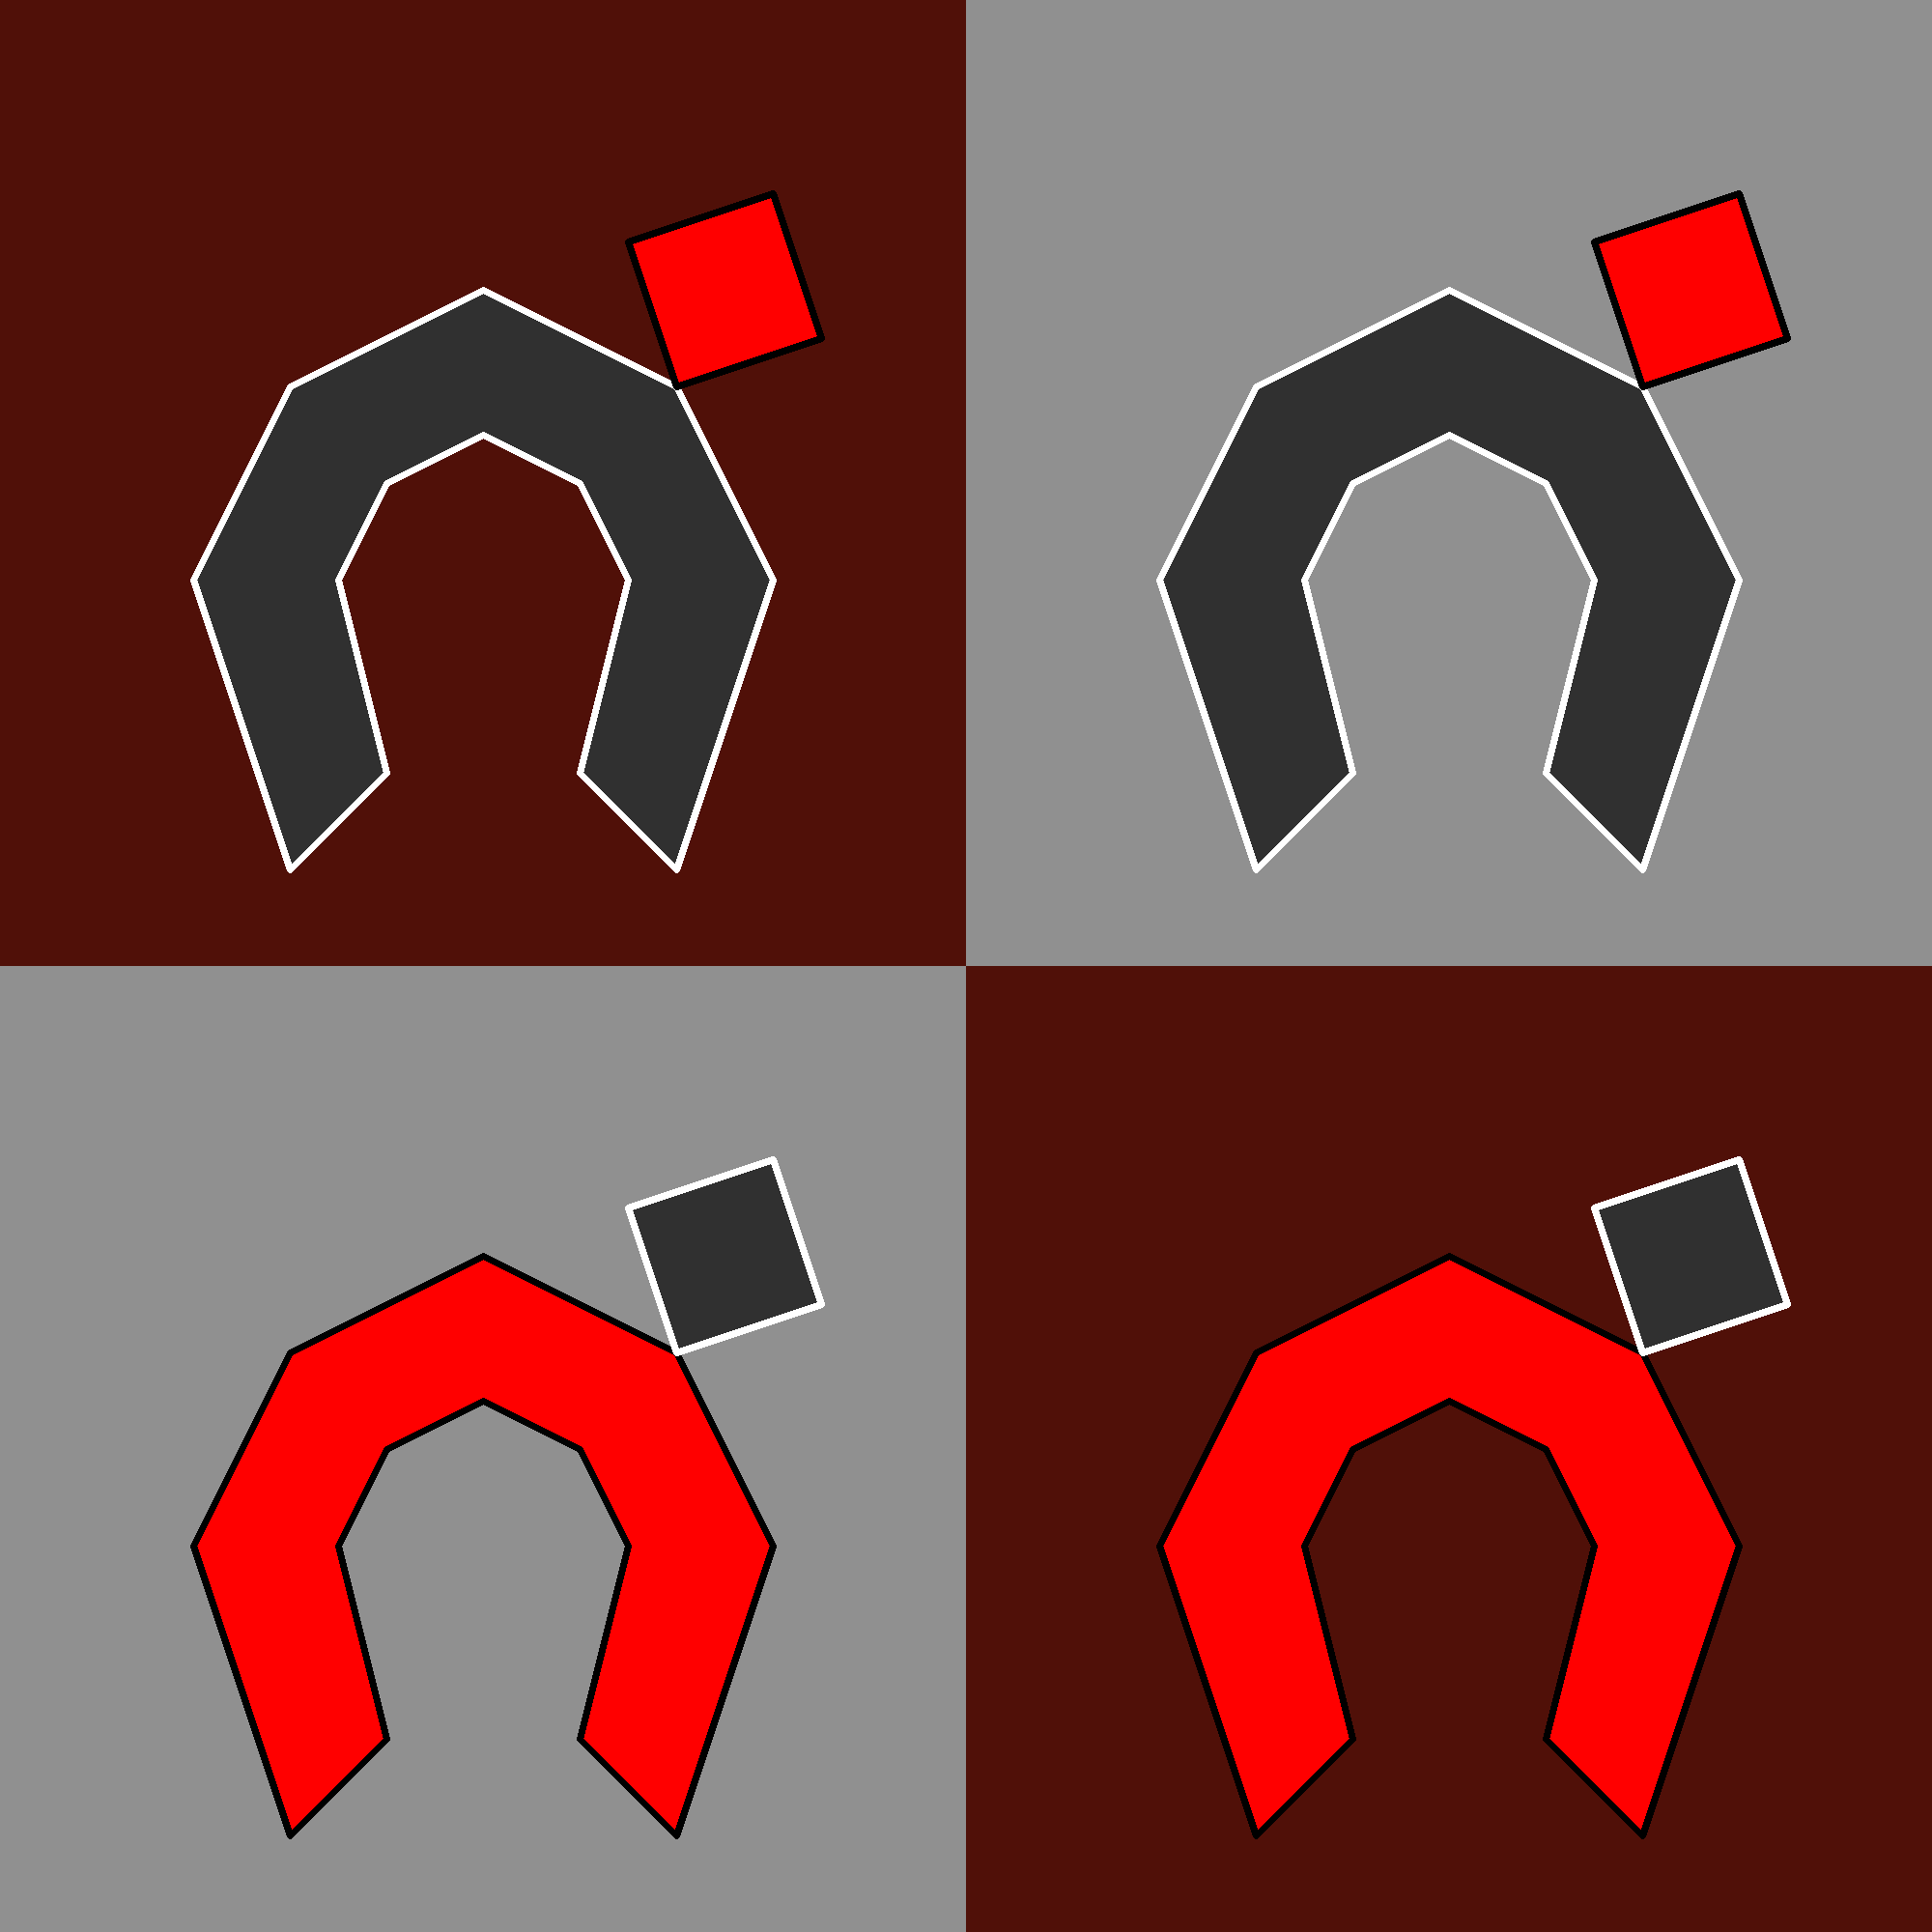
\includegraphics[width=0.4\textwidth, keepaspectratio=true]{pieces/12_centaur.png}
\caption{Centaur}
\label{fig:12_centaur}
\end{wrapfigure}

\clearpage % ..........................................................

\section*{Initial setup}
\addcontentsline{toc}{section}{Initial setup}

Initial setup can be seen in image below:

\noindent
% \begin{figure}[t]
\begin{figure}[h]
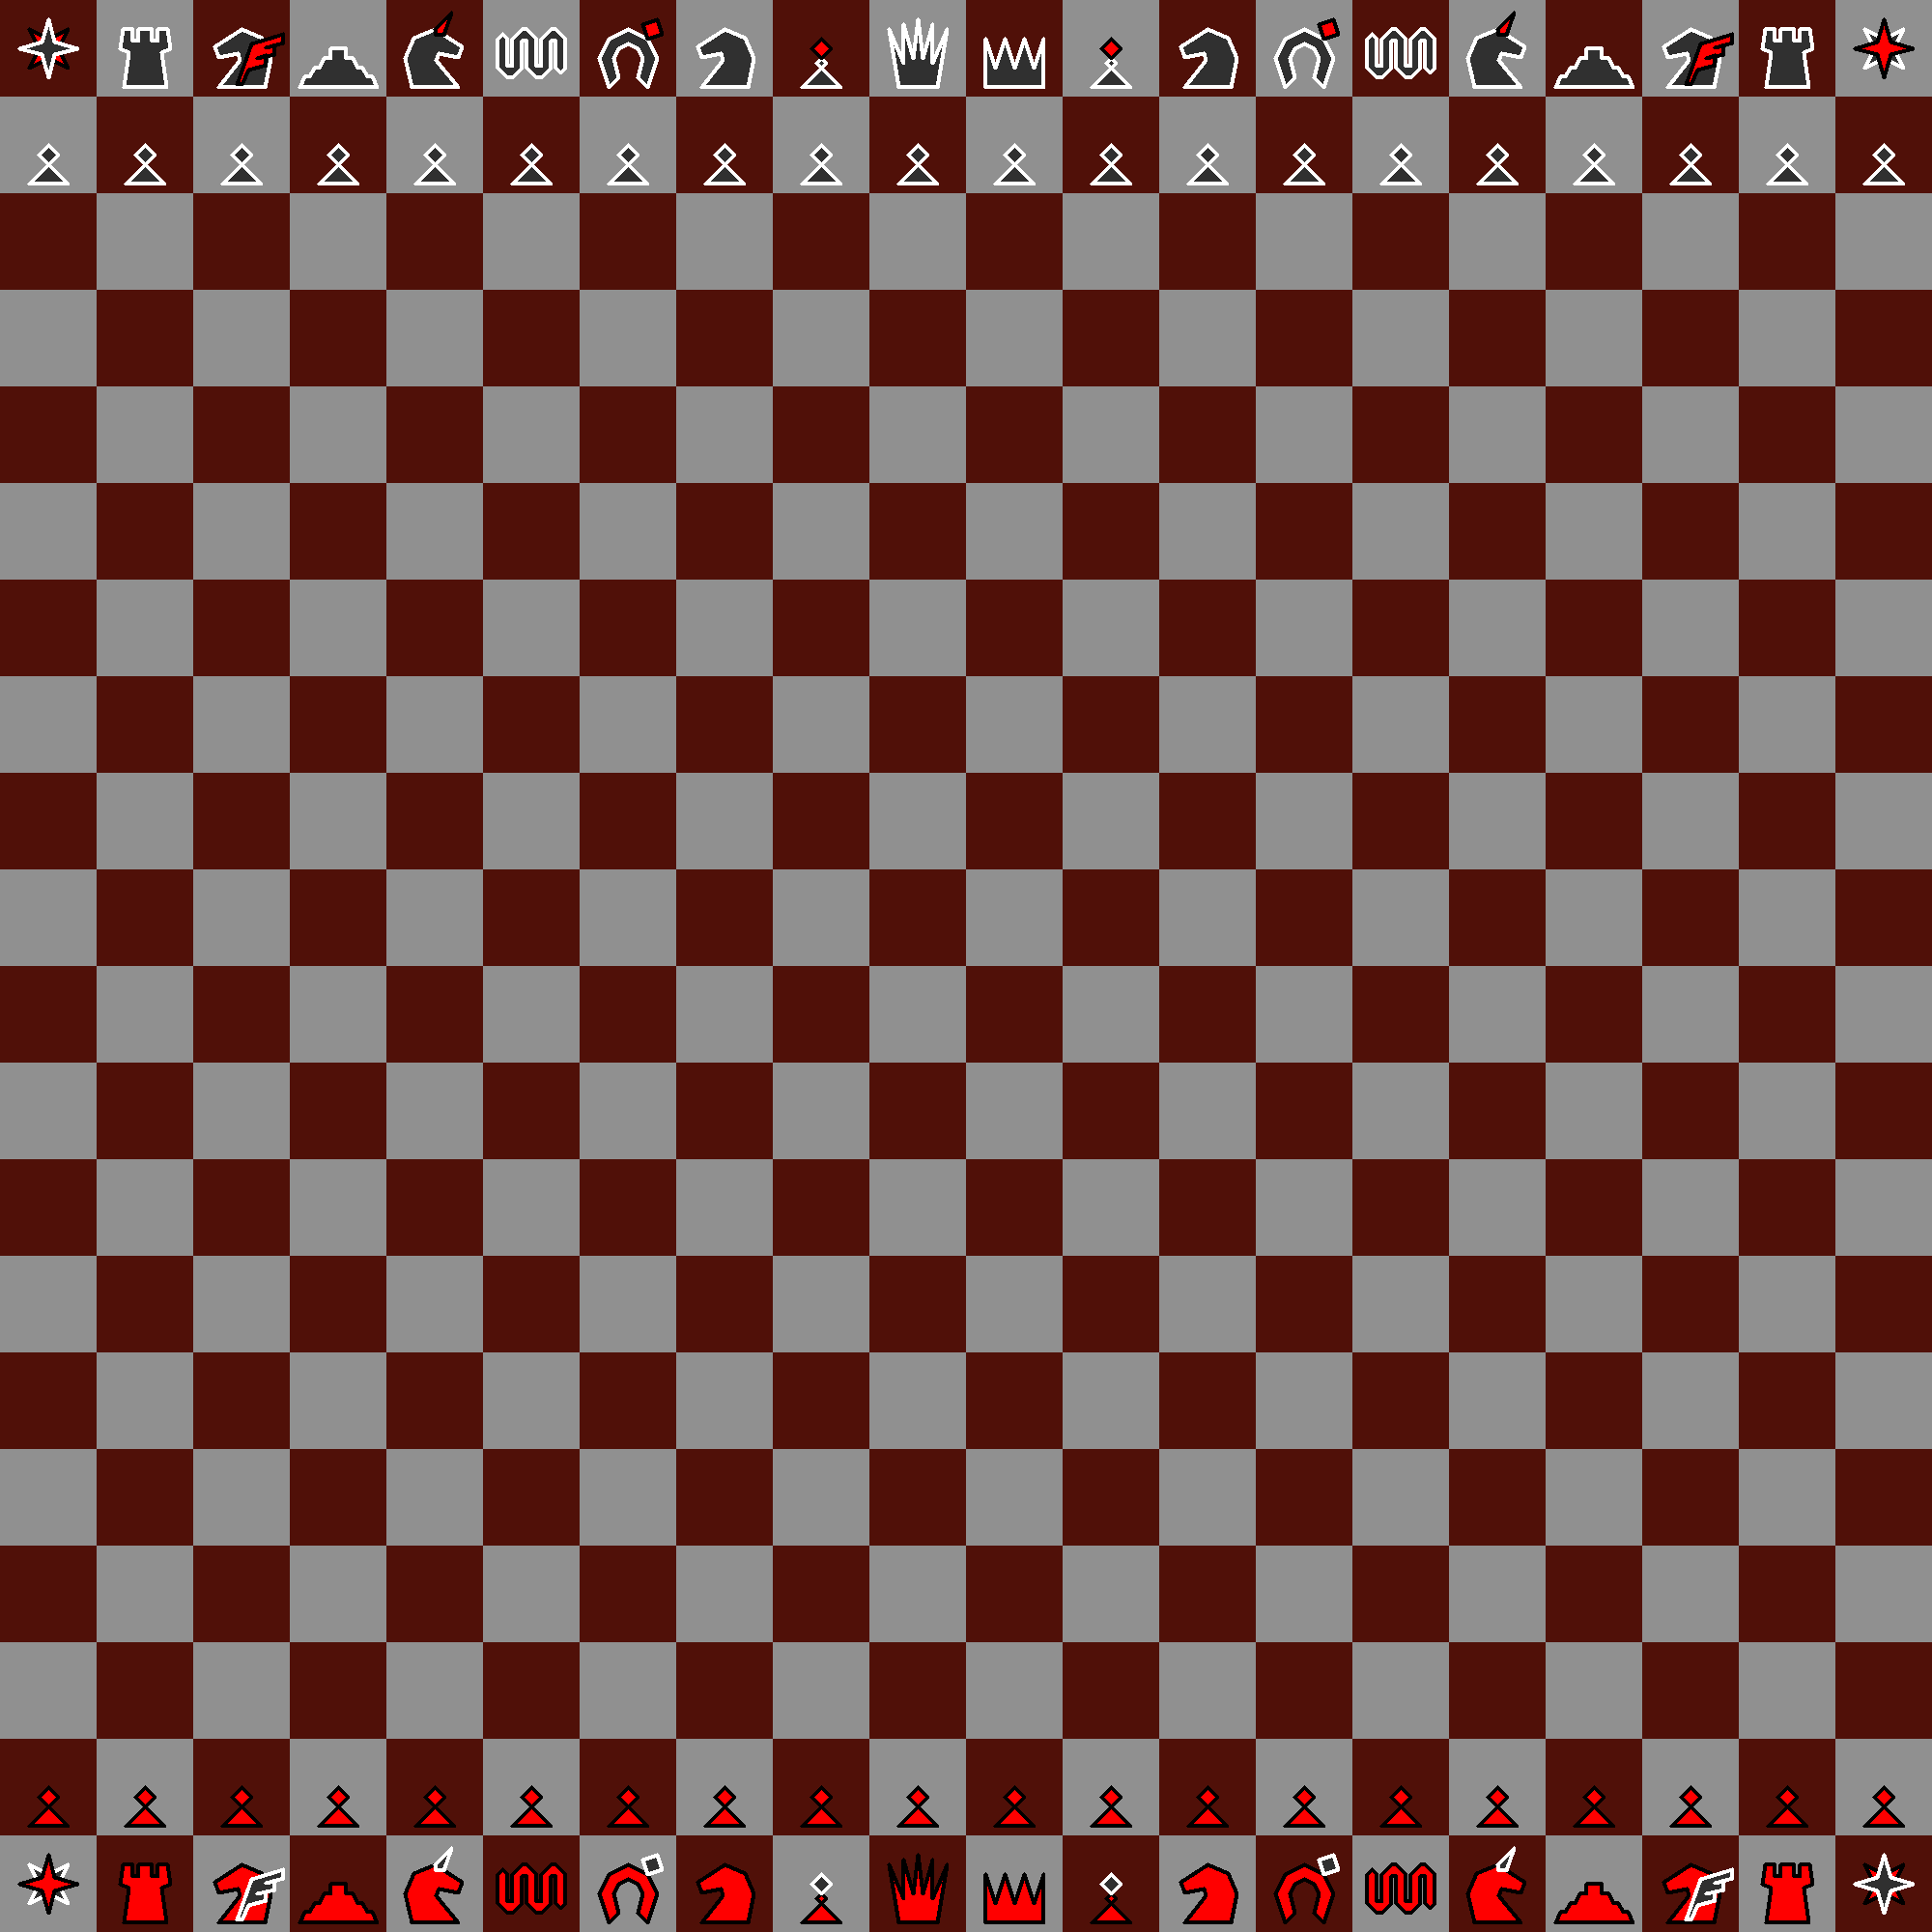
\includegraphics[width=1.0\textwidth, keepaspectratio=true]{boards/14_hemera_s_dawn.png}
\caption{Hemera's Dawn board}
\label{fig:14_hemera_s_dawn}
% \centering
\end{figure}

\clearpage % ..........................................................
% ----------------------------------------------- Hemera's Dawn chapter
